\documentclass[11pt]{article}
\usepackage[top=0.75in, bottom=0.8in, left=0.75in, right=0.75in]{geometry}
\usepackage{amsmath,amssymb}
\usepackage{graphicx}
\graphicspath{{../}{./}}
\usepackage[expansion=false]{microtype}
\usepackage[hidelinks]{hyperref}
\usepackage{enumitem}
\setlist{nosep,leftmargin=1.4em}
\setlist[itemize]{label=$\bullet$}
\setlength{\parskip}{0.4em}
\setlength{\parindent}{0pt}
\makeatletter
\renewcommand\paragraph{\@startsection{paragraph}{4}{\z@}{0.7ex \@plus 0.3ex}{-1em}{\normalfont\normalsize\bfseries}}
\makeatother
\setlength{\abovedisplayskip}{6pt}\setlength{\belowdisplayskip}{6pt}

\newcommand{\E}{\mathbb{E}}

\begin{document}

\noindent{\large\bfseries Adaptive Negotiation Training Through Human-Centered RL}\\[2pt]
Yash Ravipati, Mahdi Nassereddine, Vincent Song \textperiodcentered{} CS2822r, Fall 2026

\section{Research question}

In this project, we test whether rehearsing a negotiation with an LLM coach can improve human performance. We invert the usual reinforcement learning (RL) setup and treat the human as the `model’ being optimised. We ask whether a user’s negotiation performance improves over several rounds of LLM-synthesised rehearsals followed by feedback. We state the question more formally and describe our system setup below. The formalism itself has been a sizeable part of our progress since Checkpoint 1.

\paragraph{Scope of the present evidence.}
We have not conducted a human pilot. The results below evaluate simulated LLM
negotiators and distinguish improvements over their own baselines from improvements
over an existing coaching method. Although several conditions improve their mean
score after practice, neither personalized prompt refinement nor varied practice has
yet demonstrated reliable superiority over ordinary post-session reports in our
prospective comparisons. The human-learning question remains open.
A new, separately frozen corrected-core comparison found higher Sim4 scores with
five retained coaching reports than without feedback: mean paired gain $0.4094$
across four simulation replicates. This is exploratory evidence from two concession
profiles, not validation of the full six-weakness population or human improvement.
A prospective eight-replicate confirmation on previously unused Cedar also found
higher scores with ordinary reports: paired gain $0.1968$, exact two-sided
sign-flip $p=0.03125$. This supports a narrow score benefit in the tested simulator;
the designated weakness counts did not improve.

\paragraph{Implementation defect discovered after these experiments.}
\textbf{The intended six-weakness LLM personas were not correctly specified.}
The learner prompt serialized numeric tendencies under opaque IDs such as
\texttt{error:1}, without a dictionary explaining which behavior each ID represented.
This omission is present in the historical learner implementation as well as the
frozen implementation used for the pre-audit experiments. Therefore those results do
\emph{not} validate training learners with the intended named weaknesses, and should
not be presented as evidence for that personalized-training claim. The historical tables retain
the observed scores under the defective prompt; they are not results from a corrected
simulator. The omission does not establish the cause of the negative comparisons.
The separate scripted policy implements named behaviors in code and is not affected
by this prompt defect. Corrected prompts, behavioral calibration and new controls
are required before testing the intended LLM-persona hypothesis again.
The subsequent correctness audit repaired the missing definitions; its fresh
integration tests, persona diagnostics and exploratory transfer evaluation are
reported separately below. They do not retroactively validate the earlier experiments.

\paragraph{1. The case $c$.}
The case is the negotiation the user uploads. Formally, a case is the tuple
\begin{equation}
c = \big( \mathcal{A},\; p^{\mathrm{U}},\; p^{\mathrm{C}},\; W^{\mathrm{U}},\; W^{\mathrm{C}} \big), \qquad \mathcal{A} = \mathcal{O}_1 \times \dots \times \mathcal{O}_L,
\end{equation}
whose parts are as follows. The case has $L$ \emph{issues} to be agreed; in a job-offer negotiation between a candidate and an employer, the issues might be salary, start date, and whether remote work is allowed. Each issue $\ell$ has a set of options $\mathcal{O}_\ell$, which may be finite, such as $\mathcal{O}_3 = \{\text{yes}, \text{no}\}$ for remote work, or continuous, such as $\mathcal{O}_1 = [\$100\text{k}, \$150\text{k}]$ for salary. An \emph{agreement} $a \in \mathcal{A}$ picks one option for every issue, for example $a = (\$120\text{k}, \text{October start}, \text{yes})$. The functions $p^{\mathrm{U}}, p^{\mathrm{C}} : \mathcal{A} \to \mathbb{R}$ are the \emph{point tables} of the user and the counterpart: each says how many points that side earns from each agreement, and each side sees only its own. The candidate might earn $p^{\mathrm{U}}(a) = 4500$ points from the agreement above. Finally, $W^{\mathrm{U}}$ and $W^{\mathrm{C}}$ are the \emph{walk-away values}, the points each side receives if no agreement is reached; a candidate holding a competing offer might have $W^{\mathrm{U}} = 4000$.

\paragraph{2. The rehearsal and its score.}
A rehearsal is one negotiation of the case between the user and an LLM counterpart, and it produces a transcript. Formally, the transcript is the tuple
\begin{equation}
\tau = \big( y_1, \dots, y_N;\; a^{*} \big), \qquad N_{\mathrm{U}}(\tau) \le 20, \qquad a^{*} \in \mathcal{A} \cup \{\varnothing\},
\end{equation}
where $N_{\mathrm{U}}(\tau)$ counts user moves, $y_k$ is the $k$-th message (text, optionally with a formal offer of an agreement), and $a^{*}$ is the agreement reached, or $\varnothing$ if there was none. Messages alternate between the user and the counterpart. The counterpart's text is written by the language model, but its offers obey a \emph{concession schedule} $L(k)$, the lowest number of its own points it will accept at message $k$: it never offers or accepts an $a$ with $p^{\mathrm{C}}(a) < L(k)$. We score a rehearsal by the share of the available gains the user captured:
\begin{equation}
R(\tau) = \frac{p^{\mathrm{U}}(a^{*}) - W^{\mathrm{U}}}{P^{\star} - W^{\mathrm{U}}}, \qquad P^{\star} = \max \big\{ p^{\mathrm{U}}(a) : a \in \mathcal{A}_{\mathrm{feas}},\ p^{\mathrm{C}}(a) \ge W^{\mathrm{C}} \big\},
\end{equation}
where $\mathcal{A}_{\mathrm{feas}}$ is the subset satisfying both roles' hard constraints. The numerator is what the user gained over walking away, and $P^{\star}$ is an upper bound over feasible agreements meeting the counterpart's walk-away value; it does not guarantee acceptance under the counterpart's current schedule. A rehearsal without a deal scores $R = 0$, and $R < 0$ if the user accepts a deal worse than walking away. The transcript $\tau$ is simply the full exchange, for instance ``Candidate: I was hoping for $\$130$k. Employer: We can do $\$115$k with an October start. \dots''. The index $t = 0, 1, \dots, K-1$ counts rehearsals within one user's training run, so $\tau_t$ is the transcript of the $t$-th rehearsal.

\paragraph{3. The setting $\sigma$.}
The setting is everything the coach controls about one rehearsal. It has two parts: a difficulty tier, from 1 to 5, which sets how hard the counterpart bargains, and a \emph{focus}, which names the one mistake the rehearsal should train. A focus changes how the counterpart behaves, which moments the feedback leads with, and what the preparation notes stress. For example, the setting (tier 3, focus ``conceding first'') produces a moderately tough counterpart that holds its position until the user moves, so the user meets the situation they tend to mishandle. Formally,
\begin{equation}
\sigma = (\mu, f), \qquad \mu \in \{1, \dots, 5\}, \qquad f \in \{1, \dots, J\} \cup \{\varnothing\},
\end{equation}
where $\mu$ is the tier, $f$ is the index of the mistake to focus on (defined below), and $f = \varnothing$ means no focus. Each tier fixes a concession schedule $L_\mu$, with higher tiers opening higher and conceding more slowly. The example setting is $\sigma = (3, \text{conceding first})$.

\paragraph{4. The user's state $s$.}
The coach needs a description of the user that names their mistakes and can be estimated from a few rehearsals. We therefore describe the user before rehearsal $t$ by a vector of probabilities,
\begin{equation}
s_t = (s_{t,1}, \dots, s_{t,J}) \in [0,1]^J, \qquad s_{t,j} = \Pr(\text{user makes mistake } j \mid \text{a chance to make it arises}).
\end{equation}
Each mistake is detected by code in the transcript, along with its chances. We target $J = 6$ mistakes. \emph{Conceding first} is making the first concession before the counterpart has made any; every concession by the user is a chance to make it. An \emph{unreciprocated concession} is conceding again when the counterpart has not conceded since the user's last concession. \emph{Anchoring on their number} is answering the counterpart's opening offer with a counteroffer closer to their number than to one's own best outcome. \emph{Accepting low} is accepting an agreement that captures little of the available gains, meaning a score $R$ (defined above) below a fixed threshold. \emph{Ignoring an issue} is never raising or varying an issue that one's own point table values; each such issue is a chance once per rehearsal. A \emph{dominated offer} is proposing an agreement when another agreement already on the table gives both sides at least as many points. Acting on key facts of the case and building rapport are tracked the same way. The state is hidden, and it changes as the user learns. A user is therefore the tuple
\begin{equation}
u = \big( s_0,\; \mathrm{Learn}_u \big), \qquad \tau_t \sim \mathrm{Rehearse}(c, s_t, \sigma_t), \qquad s_{t+1} \sim \mathrm{Learn}_u(s_t, \sigma_t, F_t),
\end{equation}
where $s_0$ is the state before training, $F_t$ is the feedback shown after rehearsal $t$, Rehearse is the negotiation itself (the user's messages drawn so that mistake $j$ happens at rate $s_{t,j}$, the counterpart's from the language model and $L_\mu$), and $\mathrm{Learn}_u$ is how this user changes between rehearsals. $\mathrm{Learn}_u$ is unknown, and for real users it happens in their head.

\paragraph{5. The coach's belief $b$.}
The coach sees only what the detectors count. For mistake $j$ in rehearsal $t$, it observes $n_{t,j}$ chances and $m_{t,j}$ mistakes, which follow
\begin{equation}
m_{t,j} \sim \mathrm{Binomial}(n_{t,j}, s_{t,j}).
\end{equation}
Its belief $b_t$ is a Beta distribution for each $s_{t,j}$. A Beta distribution describes an unknown probability through two numbers that act like counts of past mistakes and past successes, so updating it after a rehearsal means adding the new counts. Because the user is expected to improve, older counts are shrunk by a factor $\lambda \in (0, 1]$ before the new ones are added:
\begin{equation}
b_t = \big( \mathrm{Beta}(\alpha_{t,j}, \beta_{t,j}) \big)_{j=1}^{J}, \qquad
\alpha_{t+1,j} = \lambda\, \alpha_{t,j} + m_{t,j}, \qquad
\beta_{t+1,j} = \lambda\, \beta_{t,j} + (n_{t,j} - m_{t,j}).
\label{eq:update}
\end{equation}

\paragraph{6. The coach $\pi$.}
The coach turns its belief into the next setting, and turns each transcript into feedback. Together with the belief update above, this makes the coach the tuple
\begin{equation}
\mathcal{C} = \big( b_0,\; \mathrm{Update},\; \pi,\; \mathrm{Feedback} \big), \qquad
\begin{aligned} \sigma_t &= \pi(b_t), & F_t &= \mathrm{Feedback}(\tau_t), \\ b_{t+1} &= \mathrm{Update}(b_t, n_t, m_t), \end{aligned}
\end{equation}
where $b_0$ is the starting belief, Update is equation~\eqref{eq:update}, $\pi$ is the \emph{policy} that picks the setting, and Feedback writes the report.
Feedback works by replaying the negotiation from key turns with the user's move swapped for an alternative, and reporting how much each alternative would have changed $R$.

\paragraph{Implemented policy and comparison baselines.}
We have several strategies for choosing the focus of the next negotiation rehearsal.
Greedy selects the user's main estimated weakness; adaptive does the same but gives
extra priority to areas we know less about.
Random chooses uniformly, and no focus sets no target, but all four policies use the
same difficulty schedule and receive feedback.

\paragraph{Learning objectives.}
A user's \emph{competence} is their expected score on a fixed set $\mathcal{D}$ of held-out cases and tiers, played with no focus and no feedback. Formally,
\begin{equation}
G(s) = \E_{(c,\,\mu) \sim \mathcal{D}} \big[ R(\tau) \big], \qquad \tau \sim \mathrm{Rehearse}\big(c, s, (\mu, \varnothing)\big).
\end{equation}
The coach's objective is the expected gain in competence over a training run of $K = 5$ rehearsals, averaged over users $u$. A coach that takes a typical user from $G = 0.25$ to $G = 0.40$ in five rehearsals contributes a gain of 0.15 for that user:
\begin{equation}
\max_\pi \; V(\pi) = \E_u \big[ G(s_K) - G(s_0) \big], \qquad s_K \text{ produced by running } \mathcal{C} \text{ with policy } \pi \text{ on user } u.
\end{equation}

\section{Implementation and preliminary evaluation}

\paragraph{Completed system.}
We have built a working app where users rehearse a negotiation and receive feedback
afterwards. The LLM writes the counterpart's dialogue, while code controls its offers
and concessions so that we can consistently adjust how hard it bargains. After the
session, the coach revisits key decisions and simulates alternative moves to estimate
how they might have changed the outcome. It also tracks which mistakes recur and how
many chances the user had to avoid them, building a profile that helps choose what to
practise next.\footnote{The evaluated implementation preserves the Beta prior while
discounting past evidence; equation~\eqref{eq:update} is retained as a sensitivity variant.
Sessions allow 20 user moves plus counterpart replies.}

\paragraph{Evaluation design.}
We used class materials from Simulation 3 as the case setting, from which six issues
with three options each were generated, giving 729 possible agreements. Point tables
and walk-away values were inferred for the experiment. We randomly sampled eight LLM
personas and tested all four focus-selection mechanisms on each persona. Each completed
five rehearsals per mechanism at tiers $(2,2,4,4,4)$. Performance was measured before
training and after each mechanism using $G$ as the average score on no-focus negotiations
at tiers $(1,3,5)$ on the same case. Including these assessments, the experiment comprised
280 negotiation episodes.

\paragraph{Results.}
From a shared mean baseline $G=0.3807$, we observed the following gains after practice with coaching:
\begin{center}
\begin{tabular}{lc}
\hline
Practice policy & Mean $G$ gain \\
\hline
Adaptive & 0.0871 \\
Greedy & 0.0672 \\
Random focus & 0.0549 \\
No focus & 0.0786 \\
\hline
\end{tabular}
\end{center}
The mean $G$ gain of the adaptive policy minus that of the random one was $0.0322$,
but that of adaptive minus that of no focus was $0.0085$.
Note that during our development, we tentatively selected an uncertainty bonus of
$\kappa=0$ because it gave the largest reduction in simulated error cost, so adaptive
and greedy used the same selection rule, and their differences here reflect model randomness.

The paired 95\% persona-bootstrap interval for adaptive minus no focus is
$[-0.0303,0.0436]$. Thus this preliminary experiment does not establish a benefit
from adaptive targeting. All conditions receive feedback; a positive before/after
gain cannot isolate coaching from practice, retained context, or model randomness.
This study's probes are on the training case, not a test of cross-case transfer.

\paragraph{Controller and profiling checks.}
Separate offline experiments found zero economic-schedule violations in 7,960 primary
scripted sessions and monotonically harder tiers. This validates the controller's
specified behavior, not its human realism. In 128 grounded scripted users, adaptive
practice had mean competence gain $-0.0059$, interval $[-0.0163,0.0046]$; an abstract
Binomial oracle improved its stipulated error-cost objective, which is a different
outcome. Profiling was checked against empirical error rates from 30 additional
reference sessions for each of 64 scripted users. Coverage was particularly poor
for unreciprocated concessions (65.6\%) and higher for ignoring an issue (98.4\%).
The reference rates themselves have Monte Carlo error. These checks do not justify
interpreting planted behavior parameters as calibrated human error probabilities.

\section{Personalized coaching memory and transfer}

\paragraph{From a latent learning rule to an executable intervention.}
For an LLM surrogate, we implement adaptation through retained post-session memory
$M_{u,t}$, rather than manually decreasing the user's error probabilities:
\begin{equation}
M_{u,t+1}=\operatorname{Coach}(D_{u,0:t},M_{u,t}),\qquad
\tau_{u,t+1}\sim\operatorname{LLMUser}(c,s_{u,0},M_{u,t+1},\sigma_{t+1}),
\end{equation}
where $D$ contains completed practice transcripts and feedback. Persona parameters
and model weights remain fixed. Each assessment starts a fresh actor with its
assigned persona and frozen memory, and provides no assessment feedback. Consequently,
the measured effect is contextual adaptation, not durable learning without memory.
Here ``persona'' denotes a sampled prompt configuration, not a validated six-weakness
learner: the missing codebook described above prevents that stronger interpretation.
The Binomial model above is an idealization: scripted action propensities and LLM
persona instructions need not equal realized conditional detector error rates.

Our prompt-refinement approach is inspired by GEPA's use of execution traces to
propose and evaluate prompt changes~\cite{gepa}. We test bounded reflective memories
and development-based selection; we do not implement GEPA's full population search,
Pareto selection, or recombination. A personalized prompt is therefore a testable
intervention, not a presumed improvement.

\paragraph{Initial Sim4 transfer study.}
Eight fixed personas completed five Sim3 rehearsals in each of three conditions:
accumulated reports; a reflective card containing conditional rules; and a card
revised after the learner applied its lesson to a fictional analogy. Conditions
were run in randomized order, with no focus and tiers $(2,2,4,4,4)$. Frozen memories
were assessed on Sim4 at tiers $(1,3,5)$; a generic untrained advice card was an
additional reference. The study comprised 216 Sim3 and 120 Sim4 episodes.
Sim4 was unused for selection in this study. Once its results had been inspected,
we treated it as a revisited development benchmark in every subsequent experiment.
It cannot be relabeled an untouched holdout for the later methods.

\begin{center}
\begin{tabular}{lrrl}
\hline
Sim4 condition & Final $G$ & Gain & 95\% interval for gain \\
\hline
Five reports & 0.5714 & $+0.0750$ & $[0.0208,0.1307]$ \\
Reflective card & 0.5797 & $+0.0833$ & $[0.0172,0.1313]$ \\
Application/correction & 0.5146 & $+0.0182$ & $[-0.0771,0.0948]$ \\
Generic advice, untrained & 0.5104 & $+0.0141$ & $[-0.0521,0.0693]$ \\
\hline
\end{tabular}
\end{center}
The shared baseline was $G=0.4964$. Reflection minus reports was only $+0.0083$,
with paired interval $[-0.0552,0.0662]$; this establishes neither superiority nor
equivalence. On the training case, reports gained $0.0483$, versus $-0.0028$ for
reflection and $0.0057$ for application/correction. Cards retained about 1,508
characters versus 16,508 for reports (91\% fewer), but this is a context-size
comparison, not proof of equal effectiveness or lower total API cost. The
application exercise also adds model calls. All 336 episodes agreed above or at
walk-away, with zero counterpart schedule violations.

\paragraph{Matched-history development.}
To separate memory format from differences in the practice trajectory, the next
experiments reused the exact same five report-guided Sim3 histories within each
persona. We compared a workbook combining a decision procedure, personal rules and
two worked historical comparisons; the procedure alone; and ablations that removed
examples or combined instructions with all reports. Further variants selected
lessons by modeled terminal counterfactual credit or added an exact own-value
worksheet. No alternative received assessment feedback during preparation.

All eight development personas were evaluated on hiring and revisited Sim4, with
cases and tiers averaged within persona. Exact reused control episodes were
hash-checked and counted once. Before the latest follow-up, the exploratory comparison was:
\begin{center}
\begin{tabular}{lrl}
\hline
Memory, relative to reports & Paired difference & Pointwise 95\% interval \\
\hline
Reflective card & $-0.0571$ & $[-0.0967,-0.0207]$ \\
Workbook & $+0.0001$ & $[-0.0413,0.0429]$ \\
Fixed procedure & $-0.0116$ & $[-0.0547,0.0267]$ \\
Workbook without examples & $-0.0210$ & $[-0.0554,0.0182]$ \\
Reports plus procedure & $-0.0075$ & $[-0.0490,0.0304]$ \\
Terminal-credit memory & $-0.0061$ & $[-0.0387,0.0247]$ \\
Reports plus value worksheet & $-0.0068$ & $[-0.0319,0.0302]$ \\
\hline
\end{tabular}
\end{center}
Selecting each persona's best memory on hiring also failed to improve pooled Sim4
transfer. The terminal-credit and worksheet candidates failed the advance rule
recorded before their calls: positive mean advantage both across all eight personas
and in the separate four-person validation cohort. Neither consumed fresh-case
confirmation calls. These are repeated exploratory comparisons on known cases;
the intervals are not adjusted for multiple comparisons.
Both cohorts had been examined in earlier experiments, so the later screening rule
does not provide an independent holdout validation.

\section{Prospective comparisons on new cases}

\paragraph{Workbook confirmation.}
We froze two original synthetic cases, Harbor Analytics and Maple Festival, and
assessed seven new personas using one shared five-session reports-guided history
each. The four conditions were reports, workbook, procedure only, and workbook
without examples. Each condition was assessed at three tiers on each new case.
The primary endpoint averaged both cases within each persona. This study added
77 training-case episodes and 210 fresh-case assessment episodes.

\begin{center}
\begin{tabular}{lrr}
\hline
Condition & Final mean $G$ & Gain over baseline \\
\hline
Reports & 0.14677 & $+0.00509$ \\
Workbook & 0.14665 & $+0.00497$ \\
Fixed procedure & 0.16883 & $+0.02715$ \\
Workbook without examples & 0.13270 & $-0.00898$ \\
\hline
\end{tabular}
\end{center}
Baseline $G$ was 0.14168. The prespecified workbook-minus-reports difference was
$-0.00011$, with 95\% interval $[-0.03328,0.02972]$, $n=7$. The first case favored
the workbook and the second reversed that result. The procedure-only advantage
over reports was $+0.02206$, interval $[-0.01105,0.05690]$, a secondary inconclusive
comparison. Of 210 assessment episodes, 208 agreed and two baseline episodes ended
in impasse. There were 39 below-walk-away agreements: baseline 7, reports 10,
workbook 5, procedure 7, and no-example workbook 10. All remain in the analysis;
zero schedule violations were found. High agreement rates alone are not success.

\paragraph{Varied practice.}
After the memory comparisons, we tested changing the five-session curriculum:
two exact shared Sim3 sessions followed by hiring/Sim4/hiring, versus five Sim3
sessions. Both conditions retained five ordinary reports. This changes case
content, roles, order and report length together; it is not a matched-history
prompt-refinement comparison. Development used the eight original personas on
the now-known Harbor case, adding 24 practice and 72 assessment episodes.
Varied practice exceeded reports by $0.04167$, interval $[-0.00987,0.08662]$.
Its separate validation-cohort mean advantage was $0.02193$. This passed the
prespecified positive-mean screening rule, but neither interval established superiority.

We then froze the intervention before testing the unused Beacon Museum case.
All seven existing confirmation personas completed three new practices after
their original two-session prefix; no prior assessment feedback entered their
memories. Baseline, five-Sim3 reports, and varied-practice reports were assessed
at three tiers: 21 new practice and 63 assessment episodes.
\begin{center}
\begin{tabular}{lrrl}
\hline
Beacon condition & Final $G$ & Gain & 95\% interval for gain \\
\hline
Five Sim3 reports & 0.45330 & $+0.03388$ & $[-0.00643,0.07692]$ \\
Varied-practice reports & 0.45788 & $+0.03846$ & $[-0.01740,0.09707]$ \\
\hline
\end{tabular}
\end{center}
Baseline $G$ was 0.41941. The primary paired advantage was only $+0.00458$,
interval $[-0.04396,0.04396]$, $n=7$. Five personas improved and two worsened.
All 63 assessments agreed above walk-away; all 21 practices agreed at or above it,
with no schedule violations. The larger development advantage did not replicate
clearly. Beacon was new, but these personas had participated in the preceding
confirmation, so this is a new-case follow-up rather than fresh-persona replication.

\begin{figure}[!htbp]
\centering
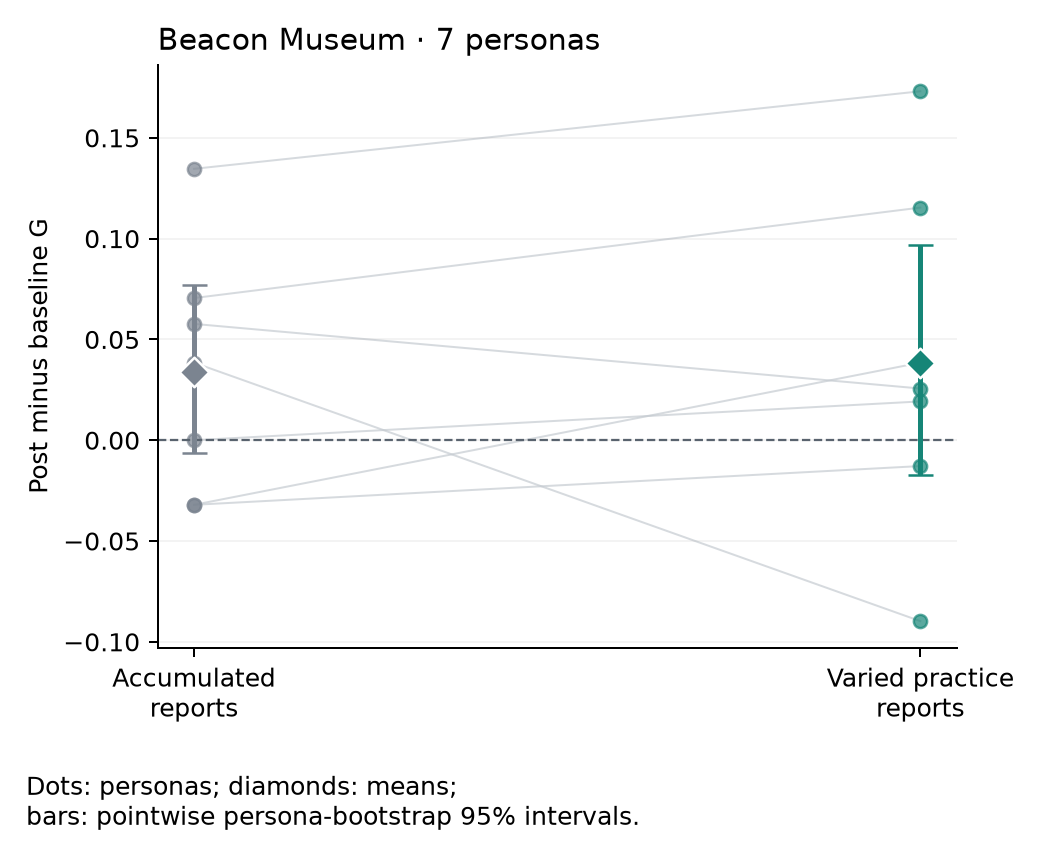
\includegraphics[width=0.68\linewidth]{results/ckpt3/consolidation-diverse-final-v1/paired_gains.png}
\caption{Beacon paired gains over baseline for all seven personas. The 95\% interval
for varied practice minus reports includes zero.}
\label{fig:beacon}
\end{figure}

% TEACHBACK_RESULTS_BEGIN
\paragraph{Latest arithmetic teach-back comparison.}
After the same five practices, the learner explained two actual own-history comparisons;
code supplied exact point-change and walk-away arithmetic, and the coach produced
one short conditional reminder while retaining all five reports. This tested a related
mechanism to the earlier unsuccessful fictional-analogy exercise. All 32 numeric
answers were already correct, so this run cannot demonstrate a benefit from repairing
arithmetic mistakes. It added 48 assessments on hiring and revisited Sim4 and reused
96 exact baseline/report episodes across the same eight development personas.

The complete paired candidate-minus-reports difference was $-0.04635$, 95\% interval
$[-0.07744,-0.01017]$, $n=8$. The second four-person cohort also had a negative mean
($-0.02532$, interval $[-0.06713,0.02400]$). Thus the candidate failed the prespecified
advance rule and performed worse in this exploratory development comparison. All
48 new assessments agreed, including two below walk-away, with zero schedule
violations or API execution failures. The frozen Cedar Warehouse case remains unused;
no final-budget calls were made for this candidate. Its 679 requests cost \$6.87.
% TEACHBACK_RESULTS_END

\section{Verification, costs, and limitations}

\paragraph{Evaluation integrity.}
For the later studies, case utilities, methods, source code, histories and
assessment memories were frozen before each relevant comparison. An independent
enumeration of legal packages recomputes the normalization denominator and every
terminal score, and checks roles, seeds, tiers, complete cohorts and memory hashes.
The implementation uses finite listed offers and hard constraints; $P^\star$ is a
feasibility bound at the counterpart's reservation value, not a guarantee of an
agreement under its actual bargaining schedule. Negative scores and impasses are
retained. Counterpart formal actions are code-controlled; its LLM generates dialogue.
The learner is Sonnet 5.5 and dialogue/coach model is Opus 5.5, using low effort.

Intervals use 2,000 persona-level bootstrap resamples. We average cases and tiers
within a persona before calculating paired differences: hundreds of episodes do
not constitute hundreds of independent learners. Intervals are conditional on
these cases and are pointwise. Each persona/method/tier has one stochastic model
rollout; seeded settings do not make provider sampling deterministic. The repeated
development search and small cohorts limit claims even when a point estimate is positive.
One provider refusal and one output truncation in development were recovered from
durable checkpoints with their costs retained. Both completed prospective studies
had no API execution failures. The earlier focus-policy experiment had runtime
repairs during recovery and is less cleanly controlled than the later frozen studies.

% COST_RESULTS_BEGIN
\paragraph{API usage and caching (reconciled after teach-back).}
The improvement work comprises 947 new episodes across 15 distinct synthetic personas,
13,566 API requests, 86.45 million input tokens including cache activity, and
5.11 million output tokens. Its recorded usage-based cost is \$128.64. Cumulative
checkpoint-3 costs, including earlier work, are:
\begin{center}
\begin{tabular}{lrrr}
\hline
Ledger & Recorded cost & Authorized cap & Remaining \\
\hline
Development & \$91.86 & \$110.00 & \$18.14 \\
Final evaluation & \$87.08 & \$110.00 & \$22.92 \\
Total checkpoint 3 & \$178.94 & \$220.00 & \$41.06 \\
\hline
\end{tabular}
\end{center}
Both caps were explicitly raised from \$100 to \$110 without resetting charges.
No requests remain unresolved in these two ledgers, and no paid run remains active.

Stable role-projected case/persona prefixes are cached separately from changing
coaching, and growing transcripts retain reusable prefix boundaries. Five-minute
cache reads covered 83.16\% of improvement-work input tokens. The same token volume
without caching would cost approximately \$302.06 versus \$128.64 in usage receipts:
estimated savings \$173.43. These are accounting comparisons, not randomized cache
experiments. Generated replies are not memoized; independent assessments retain
independent sampling. Cache-write charges and failed/retried requests remain accounted
for; per-request rounding explains the \$0.00582 receipt/ledger difference.

The separate historical ledger contains \$65.34 of known usage and nine uncertain
requests retaining \$68.09 in conservative upper bounds. Those bounds are not
confirmed spending. The three-ledger known total is \$244.28, plus that historical
uncertainty. All amounts are provider-usage estimates, not invoices.
% COST_RESULTS_END

\paragraph{What the simulations cannot establish.}
The point tables and walk-away values for class-derived cases are analyst assumptions;
the original synthetic cases also use stipulated utilities. Scores do not measure
real-world welfare or validate those assumptions. Private sheets remain separated
during negotiation; model-based post-session counterfactuals are uncertain estimates,
not observed effects of taking an alternative. A negotiation concession can be
productive, so reducing a detector count is not automatically improving terminal return.
The scripted counterfactual continuation policy may differ from the actual learner.
There is no human pilot, human annotation-agreement study, validated human-error
distribution, or evidence of human transfer. More generally, retained advice may
change an LLM's next response without teaching the lasting skill that the human
training objective requires.

\paragraph{Research conclusion and next step.}
The completed evidence supports a working, auditable simulation platform and a
controlled comparison of coaching choices. It does not support declaring the new
prompt-refinement methods or adaptive curriculum better than ordinary reports.
The persona-specification defect further prevents interpreting these comparisons
as a valid test of training the intended weakness-conditioned learners.
We retain reports as the reference method. Further improvement should target a
specific observed decision failure, use a development gate, and test the frozen
intervention on more fresh cases and personas. A larger preregistered comparison
and, ultimately, a human study are needed for stronger claims. We will not tune
against Sim4 or the other observed confirmation outcomes and continue calling
them untouched tests.

\paragraph{Corrected-system audit and fresh integration test.}
The repaired learner prompt supplies each weakness's name and behavioral definition
beside its unchanged numeric frequency. The audit also corrected the joint-efficiency
reference to obey hard constraints and added rejection of non-finite utilities,
duplicate IDs and invalid constraint references. The primary normalized-surplus
denominator already respected constraints. A follow-up input audit also rejected blank
IDs and extra unlisted point-table entries; the standalone scorer now checks the public
option catalog even if a point table is later mutated. All 218 offline tests pass.

A fresh live smoke test identified and explained all six intended weaknesses correctly.
Two learners then each completed baseline, feedback and reassessment on the public hiring
case: four agreements, no below-walk-away outcomes and no schedule violations. Every
episode scored $R=0.230769$, so no improvement was observed. This tests comprehension
and integration, not calibrated weakness frequencies or coaching efficacy. Its 60
requests cost an additional \$0.483545. The preceding cost table is the pre-audit
snapshot. Audit details are in \path{logs/ckpt3-system-audit.md}.

\paragraph{Behavioral validation of the repaired persona prompt.}
Comprehension did not establish enactment. We therefore froze a fresh 48-episode
screen: six target weaknesses, low/high settings of 0.1/0.9, two existing public
development cases (hiring and Harbor), and two matched controller seeds. All other
error settings were 0.3; awareness and rapport were 0.5. Each learner received no
feedback or preparation callout. A tier-3 rule-based counterpart exposed the target
behavior; its focus was kept separate from learner coaching. Sim4 and unused Cedar
were excluded. The primary diagnostic was the fraction of episodes exhibiting the
target error; opportunity-conditioned counts were secondary. Model sampling was not
seeded, and this small screen cannot establish calibrated probabilities.

\begin{center}
\begin{tabular}{lrrrr}
\hline
& \multicolumn{2}{c}{Episodes with error / 4}
& \multicolumn{2}{c}{Occurrences / opportunities} \\
Weakness & Low & High & Low & High \\
\hline
Conceding first & 4 & 4 & 4/14 & 5/14 \\
Unreciprocated concession & 3 & 4 & 5/14 & 7/16 \\
Anchoring & 0 & 0 & 0/4 & 0/4 \\
Accepting low & 0 & 0 & undefined & undefined \\
Ignoring an issue & 0 & 0 & 0/22 & 0/22 \\
Dominated offer & 2 & 2 & 4/27 & 3/27 \\
\hline
\end{tabular}
\end{center}

Only unreciprocated concession moved in the intended direction on the primary
measure; the prespecified six-control screening gate failed. Accepting low had
zero detector opportunities in both groups, so its conditional rate is undefined,
not zero. Opportunities depend on the learner's actions, and the dominated-offer
detector uses both utility tables offline while the learner sees only its own.
These results do not validate a six-dimensional weakness-conditioned simulator.
Further coaching-efficacy claims require behavioral calibration or a design based
on measured baseline failures, rather than presumed planted error frequencies.

All 48 sessions agreed, with no below-walk-away outcomes, missing annotations or
schedule violations. Independent enumeration verified terminal scores. The screen
used 351 requests and cost \$1.968971; 86.5\% of its input tokens were cache reads.
Together with the smoke test, the audit evaluations cost \$2.452516. Cumulative
checkpoint-3 usage through this screen was \$181.393019
(development \$94.310884; final \$87.082135),
with no unresolved requests in those ledgers and both \$110 caps unchanged.

\paragraph{Controlled persona diagnostics.}
We next used an original three-issue diagnostic case with authored prefixes that
admit both an error-producing and an error-avoiding legal action for each target.
Each cell below contains the number of observed error events at low/high settings,
out of four independent API responses per setting. The advance rule was fixed at
at most one low-setting event and at least three high-setting events for every target.
These are one-decision diagnostics, not full negotiations or learning outcomes.

\begin{center}
\small
\begin{tabular}{lrrrrr}
\hline
& V1 definitions & V1 concrete & V2 definitions & V2 concrete & V3 intent \\
\hline
Conceding first & (2,4) & (3,4) & (0,4) & (2,4) & (0,4) \\
Unreciprocated & (4,4) & (1,4) & (4,4) & (2,4) & (0,4) \\
Anchoring & (0,0) & (0,0) & (0,0) & (0,2) & (0,2) \\
Accepting low & (0,0) & (0,0) & (0,0) & (0,2) & (0,0) \\
Ignoring an issue & (0,0) & (0,0) & (0,0) & (0,0) & (0,2) \\
Dominated offer & (0,0) & (0,0) & (0,0) & (0,0) & (0,0) \\
\hline
\end{tabular}
\end{center}

Each pair is (low-setting events, high-setting events), each out of four responses.
V1 set non-target
weaknesses to zero, which can create conflicting instructions: a dominated offer
in its prefix is necessarily also a first concession. V2 therefore left non-target
frequencies unspecified. ``Concrete'' adds situation-specific enactment descriptions.
V3 adds a private categorical behavioral intent and one-sentence effect before the
formal action; the note is removed from the public move, and scoring uses the action
rather than self-reported intent. All variants retained role information boundaries.
Manual inspection of V1's 16 issue-neglect responses agreed with the issue-raising
tags; this is an assistant audit, not human inter-rater reliability.

V1 and V2 each used 96 responses; V3 used 48. None passed the six-control gate.
V3 did pass the two concession controls (zero low versus four high events each),
providing a limited basis for testing those two explicitly specified weaknesses.
The three diagnostics cost \$0.742084 across 280 requests including annotations.
Their observed variation and overlapping detectors further caution against treating
the six initial frequencies as independent calibrated error probabilities.

\paragraph{Exploratory corrected transfer evaluation.}
We separately froze a transfer comparison limited to the two concession profiles
that passed V3's controlled diagnostic; this does not satisfy the original six-control
gate. Four simulation replicates used two runs per profile, with the target initial
frequency fixed at 0.9 and other weaknesses unspecified. Each completed five Sim3
practice sessions at tiers 2,2,4,4,4, receiving an ordinary post-session LLM report
after each. The learner used concrete enactment and private intent; code never updated
its trait values. A rule-based counterpart supplied deterministic formal actions and
templated dialogue, while Opus generated the debriefs.

After freezing all five-report memories, each replicate was assessed on Sim4 at tier 3
with and without those reports, using the same controller seed and randomized arm
order. The primary comparison is the paired difference in normalized surplus $R$.
Sim4 supplied no practice, feedback or tuning in this run; it remains a revisited
benchmark because of earlier studies. There are 20 practice episodes and eight test
episodes. Four replicates from two prompt profiles, inferred case utilities and
incomplete full-session behavioral calibration limit interpretation.

\begin{center}
\begin{tabular}{lrrr}
\hline
Profile / replicate & No feedback & Five reports & Difference \\
\hline
Conceding first / 1 & 0.6000 & 0.7500 & +0.1500 \\
Conceding first / 2 & 0.6000 & 0.7500 & +0.1500 \\
Unreciprocated / 1 & 0.0625 & 0.7500 & +0.6875 \\
Unreciprocated / 2 & 0.2375 & 0.8875 & +0.6500 \\
\hline
Mean & 0.3750 & 0.7844 & +0.4094 \\
\hline
\end{tabular}
\end{center}

Every replicate improved. The paired empirical-bootstrap 95\% interval is
$[0.1500,0.6688]$, but the exact two-sided sign-flip reference gives $p=0.125$;
four replicates cannot establish a general training benefit. The designated
concession errors did not occur in either Sim4 assessment arm, so this does not
demonstrate their remediation. Their occurrence was sparse during practice too:
two target-error events across the 20 sessions. The positive result concerns
negotiation scores under this frozen comparison, rather than a validated causal
mechanism for correcting the specified weaknesses.

All 28 negotiations reached agreements, with no below-walk-away outcomes, schedule
violations or missing annotations. Independent exhaustive scoring, transcript replay,
memory hashes and source hashes verified the complete cohort. The evaluation used
217 requests and cost \$2.439023. Total spending since the audit authorization is
\$5.633623, including the smoke test, behavioral screen and controlled diagnostics.
Cumulative checkpoint-3 known usage is \$184.574126 (development \$96.924150;
final \$87.649976), with no unresolved requests in those ledgers. Both cumulative
caps were \$110 at the end of this pilot. These usage estimates are not a provider invoice.

\paragraph{Prospective confirmation on a fresh case.}
Following the exploratory Sim4 result, we froze the same actor and coaching method
for eight new simulation replicates, four per concession profile, on Cedar Warehouse.
Cedar's case file matched its original manifest hash and had no recorded prior
negotiation outcomes. Each replicate completed five fresh Sim3 practices at the same
tiers; all 40 reports were frozen before the 16 paired Cedar assessments. The learner
played the owner at tier 3, with randomized arm order and matched controller seeds.
No Cedar feedback, practice or tuning was permitted. The criterion fixed before
assessment was a positive paired mean and a two-sided exact sign-flip $p\leq0.05$,
using all eight replicates. Source comparisons verified that the actor, coaching and
training procedure matched the pilot; the test case, role, seeds and cohort changed.
These are eight stochastic replicates of two prompt profiles, not eight independently
sampled human populations. This comparison tests ordinary reports against no feedback;
it does not test personalized refinement against ordinary reports.

\begin{center}
\begin{tabular}{lrrr}
\hline
Profile / replicate & No feedback & Five reports & Difference \\
\hline
Conceding first / 1 & 0.2553 & 0.4894 & +0.2340 \\
Conceding first / 2 & 0.2553 & 0.4894 & +0.2340 \\
Conceding first / 3 & 0.2553 & 0.6170 & +0.3617 \\
Conceding first / 4 & 0.0426 & 0.4894 & +0.4468 \\
Unreciprocated / 1 & 0.2553 & 0.3191 & +0.0638 \\
Unreciprocated / 2 & 0.3191 & 0.3191 & 0.0000 \\
Unreciprocated / 3 & 0.2553 & 0.4894 & +0.2340 \\
Unreciprocated / 4 & 0.2553 & 0.2553 & 0.0000 \\
\hline
Mean & 0.2367 & 0.4335 & +0.1968 \\
\hline
\end{tabular}
\end{center}

Six replicates improved and two tied. The paired empirical-bootstrap 95\% interval
is $[0.0957,0.3059]$ and the exact two-sided sign-flip reference gives $p=0.03125$,
meeting the prespecified confirmation criterion. This is evidence for score transfer
to one fresh case under this fixed simulation setup. It does not establish general
human learning or superiority of personalized prompt refinement. Moreover, designated
target errors occurred 3 times in 16 opportunities without feedback and 4 times in
18 opportunities with reports; practice contained 15 events in 80 opportunities.
Those endogenous opportunity counts do not demonstrate weakness remediation or
validate the nominal 0.9 trait as an enacted probability. Cedar has now been assessed
and must not be described as an unused confirmation case in future studies.

Independent exhaustive scoring, transcript replay, source and memory checks passed
for all 56 negotiations. All reached agreement; none fell below walk-away values,
violated the counterpart schedule or lacked annotations. The run cost \$4.465473
across 392 requests (practice \$3.801271; assessment \$0.664202). Total known spending
since the latest audit authorization is \$10.099096, within its \$150 allowance.
Cumulative checkpoint-3 usage is \$189.039599: development \$100.725421 and final
\$88.314178, with no unresolved requests. During practice, the development cap was
raised from \$110 to \$115 within that authorization to accommodate conservative
in-flight reservations; the final cap remains \$110. These are usage estimates.

\paragraph{Reproducibility.}
Numeric results, paired rows, frozen protocols and plots are under
\path{results/ckpt3/}. The initial transfer study is \path{final-v1}; the two later
prospective studies are \path{consolidation-final-v1} and
\path{consolidation-diverse-final-v1}. Analysis scripts independently verify scoring,
and \path{scripts/summarize_improvement_costs.py} reconciles usage with durable ledgers.
Raw transcripts, original class materials, generated personal memories and secrets
remain excluded from published artifacts. Historical frozen experiments require the
pre-repair core at git revision \texttt{4613bb2}; repaired-core results are stored
separately in \path{audit-corrected-smoke-v1} and \path{persona-calibration-v1}.
The behavioral screen used core revision \texttt{e8e0820}; its strict verifier
requires that frozen implementation. The subsequent validation-only fix preserves
all five public case serializations and all 579 recorded offer scores, checked in
\path{validation_recheck.json}. The current offline suite passes 220 tests;
the live API test is excluded from that count.
Controlled diagnostics are in \path{persona-probes-v1}, \path{persona-probes-v2} and
\path{persona-probes-v3}; the new transfer comparison is \path{corrected-transfer-v1}.
Its protocol and candidate implementation were committed at \texttt{3ebd2f4} before
Sim4 assessment. \path{scripts/verify_corrected_transfer.py} independently checks
all 28 scores, controller schedules and frozen coaching memories.
The Cedar confirmation protocol and implementation are in
\path{corrected-confirmation-v1}, committed at \texttt{80e7bb7} before assessment;
\path{scripts/verify_fresh_confirmation.py} checks its complete cohort independently.

\begin{thebibliography}{1}
\bibitem{gepa}
L.~A.~Agrawal et al.
\emph{GEPA: Reflective Prompt Evolution Can Outperform Reinforcement Learning}.
arXiv:2507.19457, 2025, revised 2026.
\url{https://arxiv.org/abs/2507.19457}.
\end{thebibliography}

\end{document}
